\newpage
\section{Method} \label{Method}

\subsection{Action research} \label{action_research}

\begin{comment}
Onderzoeksvraag:
Hoe bruikbaar is Ampersand voor het ontwerpen van register-systemen door middel van het analyseren van wet- en regelgeving in de volksgezondheid en in het bijzonder de Wet-BIG
\end{comment}
We use action research to investigate the usefulness of Ampersand.
In the introduction we already mentioned that Ampersand is little used in practice.
Therefore, we apply Ampersand in practice, so that we can experience the usefulness of the method and the tool.

The way Ampersand its usability is measured along several axes.
The definition of usability according to \cite{shackel_usability_2009} is ``the capability to be used by humans easily and effectively'' and ``the effectiveness,
efficiency, and satisfaction with which specified users can achieve goals in particular environments'' is the definition given by the NEN~\footnote{\url{https://www.nen.nl/nen-iso-iec-25010-2011-en- 157265}}.
The usability attributes according to \cite{HORNBAEK200679} are measured via Effectiveness, efficiency and satisfaction.
Usability with which the NEN measures are the Appropriateness recognisability, Learnability, Operability, User error protection, Accessibility and User interface aesthetics.
\begin{comment}
Herkenbaarheid van geschiktheid (Appropriateness recognisability)
    De mate waarin gebruikers kunnen herkennen of een product of systeem geschikt is voor hun behoeften.
Leerbaarheid (Learnability)
    De mate waarin een product of systeem gebruikt kan worden door gespecificeerde gebruikers om gespecificeerde leerdoelen te bereiken met betrekking tot het gebruik van het product of systeem met effectiviteit, efficiëntie, vrijheid van risico en voldoening, in een gespecificeerde gebruikscontext.
Bedienbaarheid (Operability)
    De mate waarin een product of systeem attributen heeft die het makkelijk maken om het te bedienen en beheersen.
Voorkomen gebruikersfouten (User error protection)
    De mate waarin het systeem gebruikers beschermt tegen het maken van fouten.
Volmaaktheid gebruikersinteractie (User interface aesthetics)
    De mate waarin een gebruikersinterface het de gebruiker mogelijk maakt om een plezierige en voldoening gevende interactie te hebben.
Toegankelijkheid (Accessibility)
    De mate waarin een product of systeem gebruikt kan worden door mensen met de meest uiteenlopende eigenschappen en mogelijkheden om een gespecificeerd doel te bereiken in een gespecificeerde gebruikscontext.
\end{comment}

We are going to conduct exploratory research to measure the usability of Ampersand and according to \cite{Easterbrook} used as initial investigations of some phenomena to derive new hypotheses and build theories.
The new hypotheses to be developed relate to the usability of Ampersand.

The development of the hypothesis takes place by measuring the usability attributes.
To measure these attributes we use \acrshort{ar}~\citep{Easterbrook}.
The core of this research method is the action-oriented approach.
The researcher is part of the organization in which the research takes place where the data is collected.
It has been set up \acrshort{ar} as a joint learning process between the researcher and the \acrshort{cibg}.
The problem owner is willing to work together to both identify a problem and make an effort to solve it.
The original problem is authentic.
There is widespread discussion about the methodology, and even debate about the validity of action research as an empirical method according to~\cite{Easterbrook} because of the accusations that action research is ad-hoc.

The action consists of making a prototype and \acrshort{ca}, because that offers many opportunities to explore the usefulness of Ampersand.
We are looking into the usability of Ampersand and the action we perform is to design a prototype of the \acrshort{zorro}.
The \acrshort{zorro} is managed by the \acrshort{cibg}.
The \acrshort{cibg} is a government organization of the \acrlong{vws}.
This registration system is based on the \acrshort{big}.
This leads to the following research question:
\newline
\textbf{\acrlong{research question}}

In order to investigate the usability of Ampersand by making the prototype, it is necessary to acquire knowledge to be able to implement this.
\\To do this part of the research, we formulate the following sub-question:
\begin{enumerate}
    \item[RQ1]- \textit{\acrlong{RQ1}}
\end{enumerate}

While making the prototype, we will work with Ampersand.
In addition to registering observations, we are also interested in the results of the campaign.
Are the Concepts, Relations and Rules found recognizable for the organization, because the \acrshort{cibg} has the \acrshort{zorro} running.
\\We formulate the following sub-question:
\begin{enumerate}
    \item[RQ2]- \textit{\acrlong{RQ2}}
\end{enumerate}

The prototype is based on the \acrshort{big}.
The Ampersand method prescribes that, in this case, we should take the law as our starting point.
Now this is also the case with a traditional design, but there is an interpretation battle over the user representation.
At Ampersand, the law is taken literally as a guideline and the prototype is made on the basis of the law.
\\That leads us to the following sub-question:
\begin{enumerate}
    \item[RQ3]- \textit{\acrlong{RQ3}}
\end{enumerate}

In order to estimate the usability for the receiving organization, it is necessary to look at what the usability attributes mean for the organization.
The usefulness of the Ampersand method is not only technical, but organizational.
There are also less rational aspects in this area.
To get to the bottom of this, we will determine the strengths of using Ampersand as a registration system for the \acrshort{cibg} and detect the weaknesses of using Ampersand.
\\We formulate the following sub-question:
\begin{enumerate}
    \item[RQ4]- \textit{\acrlong{RQ4}}
\end{enumerate}

While making the prototype, we collect two types of data.
We collect observations while making the prototype and we use interviews as a source of information and make summaries of them (see appendix \ref{appendixInterviews}).
When collecting observations, we write down everything we encounter along the way.
Each observation is given a number and a date stamp (see appendix \ref{appendixLoglines}) and is directly assigned to a sub-question.
This direct assignment is based on the assumption that the observations can lead to answers to the sub-questions.
We will run both processes time-boxed.

The chosen approach of elaboration relates to the qualitative content analysis~\citep{kohlbacher_use_2006}.
The steps described are also the steps followed within this \acrshort{ar}.
During these steps we collect evidence, studying the legal texts and converting them in part to Ampersand.
During this conversion, it was always recorded which observations had been made.
The next step is to analyse case study evidence.
This includes examining, categorizing and combining data.
There are several approaches such as ~\cite{hsieh_three_2005} and \cite{mayring_qualitative_2019}, where the outcomes include reliance on theoretical propositions and thinking about alternative explanations for developing a case description.
The last step is the reporting phase, which is performed in section \ref{Conclusions}.

\subsection{Content analysis approach}\label{subsection:content_analysis_approach}
Based on research question, we cluster according to its terms (see table~\ref{tab:Category_definitions})
\begin{table}[H]
    \caption{Category definitions}
    \begin{tabularx}{\linewidth}{|X|X|}
    \hline
        \textbf{Category} & \textbf{Definition} \\\hline
        \acrshort{cat1} & \acrlong{cat1} \\\hline
        \acrshort{cat2} & \acrlong{cat2} \\\hline
        \acrshort{cat3} & \acrlong{cat3} \\\hline
        \acrshort{cat4} & \acrlong{cat4} \\\hline
        \acrshort{cat5} & \acrlong{cat5} \\\hline
        \acrshort{cat6} & \acrlong{cat6} \\\hline
        \acrshort{cat7} & \acrlong{cat7} \\\hline
    \end{tabularx}
    \label{tab:Category_definitions}
\end{table}

The purpose of content analysis is to validate the claim that we can determine the cause of Ampersand its low usage.
Research will provide predictions about variables mentioned in table~\ref{tab:Category_definitions}.
Using a directed content analysis~\citep{hsieh_three_2005}  approach, is more organized than using a conventional approach.
Where \cite{hsieh_three_2005} calls it a directed content analysis, for \cite{mayring_qualitative_2019} this is a deductive category application.
The procedure is deductive because the category system is established before coding the text. 
The categories are deduced from keywords of the main question. 
A definition has been drawn up for each category that the category must meet according table \nameref{tab:Category_definitions}.
Based on the research question, the data and the objectives of the researcher, the following strategy can be followed in labeling/coding.
The strategy starts with labeling using the predefined codes (see table~\ref{tab:Category_definitions}).
Theoretical considerations can lead to a further categories or rephrasing of categories, but the categories are not developed out of the text material like in inductive category formation.

The existing theory is that Ampersand is very suitable for application in legislation and regulations and also for use within a government organization.
The impression is that the unfamiliarity in particular stands in the way of the use and usability of Ampersand.
The collected data will show whether there are other issues than just ignorance.
That is also the way the data is classified and treated.
The content analysis performed leads to a number of claims about the usability of Ampersand.
These claims are the result of the investigation.

We collected information about observations that stood out while building the prototype.
This information is included as observations in appendix~\ref{appendixLoglines} and via interviews in appendix~\ref{appendixInterviews}.

\begin{comment}
Deductief redeneren is een top-down onderzoeksmethode. Je zoekt op basis van een generalisatie naar specifieke gevallen. Met behulp van deductief onderzoek toets je theorieën en hypothesen. Het proces bestaat over het algemeen uit vier stappen: er is een theorie (generalisering), je formuleert een hypothese, je observeert of analyseert, je bevestigt of verwerpt de hypothese.
\end{comment}

We then work with pre-formulated categories, which are derived from the main question and establish the relationship between the categories and the observations.
This step consists of a methodologically controlled assignment of the category to a text passage of the observation.
\begin{figure}[H]
    \centering
    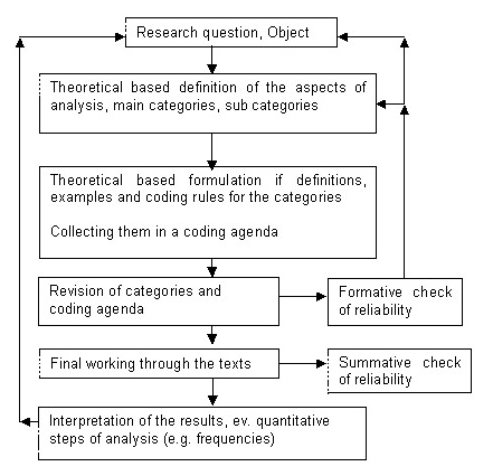
\includegraphics{Step model of deductive category application.PNG}
    \caption{Step model of deductive category application~\citep{mayring_qualitative_2000}}
    \label{fig:step-model-of-deductive-category-application}
\end{figure}

The starting point is that the usability of Ampersand is an issue.
We see this because Ampersand is rarely used.
We hypothesize that we can determine the cause of the low usage through research.

While making the prototype, we record what we notice.
The record is tagged with the date and time of the observation, so that the observation remains traceable and we hold discussions with stakeholders in the form of free interviews.

We determine the coding rules for each deductive category and  provide an example.
We then work through the observations and determine to which category the text belongs.
Here we use our chosen identification of observation.
The interview reports are divided into paragraphs and labeled with an identifier, then we determine to which category the paragraph belongs.
By means of a loop-back the theoretical basis can be further refined as can be seen in figure \ref{fig:step-model-of-deductive-category-application}.

Philip Mayring is also the founder of the website \url{https://www.qcamap.org}.
On this website, the content analysis tool allows us to perform some of the content analysis.
We define a project within QCAMap and use the method and data within our research, using the deductive approach.

After assigning the data to the category, it appears that further refinement is required within the categories.
In the section~\ref{Results} the results are logically linked so that we can also label the refined clustering and in section~\ref{section:discussion} we refer to the categorization and the refined labeling.
Here we assign the clustering to the sub-questions that we formulated earlier and are answered in this section and to answer the main question in the section~\ref{conclusions}.

\subsection{Validation}\label{subsection:validation}
The tool to be used to validate is triangulation~\citep{carter_use_2014, farquhar_triangulation_2020, runeson_guidelines_2008}.
Triangulation offers the possibility to view the source from multiple perspectives.
In addition, the engineers have the necessary knowledge and information about the application of the law and from the business perspective.
This is a way of assuring the validity of research through the use of a variety of methods to collect data on the same topic, which involves different types of samples as well as methods of data collection\footnote{\url{https://en.wikipedia.org/wiki/Triangulation_(social_science)}}.

